\chapter{Blockchain}
\label{chap:blockchain}

\section{Introduzione}
\label{sec:introduzione}

Il termine blockchain denota un particolare tipo di distributed ledger protetto mediante meccanismi crittografici.
Il distributed ledger è un log distribuito, parzialmente o totalmente replicato a cui accedono un gruppo di peer.
All’interno di una blockchain vengono memorizzate in modo permanente e immutabile una serie di informazioni verificate attraverso opportuni algoritmi di consenso.


\section{Protocolli di consenso}
\label{sec:protocolloDiConsenso}

Gli algoritmi di consenso assicurano che il nuovo blocco da pubblicare sulla blockchain sia completamente convalidato e protetto, assicurando anche che le transazioni siano valide; questi algoritmi svolgono un ruolo fondamentale nella risoluzione del problema della doppia spesa.
Il protocollo introdotto dalla prima tecnologia blockchain, cioè Bitcoin\footnote{Utilizzeremo per tutto il documento la convenzione sulla parola Bitcoin, scritta con la lettera maiuscola indicherà il protocollo Bitcoin, analogamente per bitcoin scritto con la lettera minuscola che indicherà la moneta.}, è l’algoritmo di  Proof of Work (PoW) dove, per dimostrare la validità di un blocco e il lavoro svolto, i nodi nella rete (chiamati {\it miner\/}) usano il potere computazionale per convalidare le azioni e competono tra loro in una sfida crittografica per trovare una soluzione ad un problema imposto dal protocollo.
Il vincitore ha diritto ad una ricompensa per la vincita e, se il protocollo lo prevede, a riscuotere le commissioni incluse nelle transazioni.
Il miner vincitore della sfida creerà un nuovo blocco, includendo l’hash del blocco precedente, il timestamp e le transazioni. \newline
Trasmettendo il nuovo blocco sulla rete, si può verificare un fenomeno di concorrenza: due o più nodi possono pubblicare un blocco con lo stesso hash di blocco precedente, ma contenuto completamente o parzialmente differente. Tale fenomeno viene aggirato scegliendo di lavorare con una catena di blocchi più lunga, perché in quel caso il miner avrà svolto maggior lavoro. \newline
Come ogni protocollo, i protocolli di consenso presentano vulnerabilità: in teoria, il sistema PoW può essere attaccato se un miner, da solo o in un gruppo, possiede più della metà della potenza di estrazione totale della rete e questo è anche noto come l'attacco del 51\% in cui gli aggressori creano la propria catena segreta riuscendo ad ottenere la fiducia di tutto il sistema, compromettendo le sue funzionalità.


\section{Blocchi}
\label{sec:blocchiBlockchain}

La blockchain può essere definita come una struttura ad albero con zero o al massimo un figlio; ogni blocco contiene il riferimento al blocco precedente, con cui si ottiene una relazione padre-figlio a tutti gli effetti.
Concatenando tutti i blocchi con i relativi padri, si ottiene un unico percorso con cui attraversare la blockchain, che può anche essere vista anche come una lista di blocchi concatenati singolarmente.
Il link che funge da collegamento tra i due blocchi è un puntatore crittografico chiamato comunemente {\it hash pointer \/}, generato da una funzione hash, applicata alla concatenazione delle informazioni del blocco in un preciso ordine La Tabella \ref{tab:bitcoinblock} riporta una rappresentazione generale del blocco.


\begin{table}[ht]
       \centering\small
           \begin{tabular}{l}
               \toprule
               Block\\
               \midrule
               Prova di lavoro (nonce)   \\
               Transazioni valide \\
               Timestamp \\
               Merkle Tree \\
               \bottomrule
       \end{tabular}
       \caption{Rappresentazione generale del concetto di blocco in una blockchain.\label{tab:bitcoinblock}}
   \end{table}

\begin{itemize}
  \item {\bf Nonce\/}: Esso funge da contenitore del valore usato nella PoW e il suo valore è un numero casuale che rappresenta il valore di difficoltà con cui è stato costruito il blocco.
  \item {\bf Timestamp\/}: Valore che indica la data di pubblicazione del blocco.
\end{itemize}
\leavevmode
\newline
I Merkle tree furono inventati da Ralph Merkle nel 1988, nel tentativo di costruire migliori firme digitali; questa struttura in una blockchain ha lo scopo di diminuire il costo sulla verifica delle transazioni, senza dover accedere singolarmente ad esse, e di conseguenza fornisce un modo per verificare la correttezza dell’intera blockchain.
La costruzione di questo albero inizia dalle foglie, dove ogni foglia contiene il valore hash calcolato tramite una funzione unidirezionale come MD5 oppure SHA-1, procedendo così alla creazione dei nodi interni che corrispondono alla funzione hash della concatenazione dei figli.
Utilizzando la funzione hash nella costruzione della struttura ad albero, viene garantita l’integrità delle informazioni: ciò vuol dire che, se qualche malintenzionato cambiasse il valore all’interno di una foglia, tutto il cammino radice foglia sarebbe alterato, con un cambiamento inevitabile anche della radice.
La proprietà di questa funzione vieta a chiunque di alterare le informazioni relative alle transazioni all’interno di un blocco una volta reso pubblico; ciò rende impossibile, ad esempio, aggiungere una transazione, rimuoverla o modificarla, come mostrato in Figura \ref{fig:merkletree}.

\begin{figure}[H]
\begin{center}
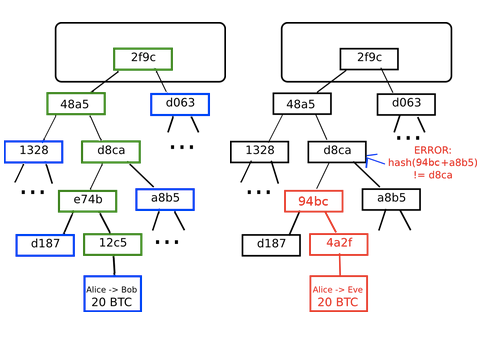
\includegraphics[width=0.6\columnwidth]{images/image-merkle-treepng.png}
\end{center}
\caption{Esempio di stato non valido per un cammino radice foglia. \cite{ethereum:paper}}
\label{fig:merkletree}
\end{figure}
